\documentclass[format=acmsmall, review=false, screen=true]{acmart}

\usepackage{booktabs} % For formal tables

\usepackage[ruled]{algorithm2e} % For algorithms
\renewcommand{\algorithmcfname}{ALGORITHM}
\SetAlFnt{\small}
\SetAlCapFnt{\small}
\SetAlCapNameFnt{\small}
\SetAlCapHSkip{0pt}
\IncMargin{-\parindent}


% Metadata Information
%\acmJournal{TWEB}
%\acmVolume{9}
%\acmNumber{4}
%\acmArticle{39}
%\acmYear{2010}
%\acmMonth{3}
%\copyrightyear{2009}
%\acmArticleSeq{9}

% Copyright
%\setcopyright{acmcopyright}
\setcopyright{acmlicensed}
%\setcopyright{rightsretained}
%\setcopyright{usgov}
%\setcopyright{usgovmixed}
%\setcopyright{cagov}
%\setcopyright{cagovmixed}

% DOI
\acmDOI{0000001.0000001}

% Paper history
\received{February 2007}
\received[revised]{March 2009}
\received[accepted]{June 2009}


% Document starts
\begin{document}
% Title portion. Note the short title for running heads
\title[The Impact of Social Inequality in AirBnB]{Who Gets the Lion's Share in the Sharing Economy: The Impact of Social Inequality in AirBnB}


\begin{abstract}
Sharing economy platforms have rapidly disrupted and transformed many traditional markets. Companies such as AirBnB, in the housing market, and Uber, in the ride-sharing space, have thrived by creating opportunities for so-called ``micro-entrepreneurs'', allowing them to leverage existing personal assets, such as a spare room or car, to generate additional income. While often heralded as an opportunity to reduce income inequality, opening opportunities through technology to a much larger segment of the population, there is however a latent concern that these platforms are in practice not as inclusive as advertised.

Looking specifically at \ab, issues of inequality and discrimination on the platform have started to attract the attention of the research community. There is however no clear understanding of how this inequality manifests itself. As a starting point, we must ask the question of who benefits the most from the use of this platform: specifically who the hosts are, their background, and what they offer.

%In this paper we study over 14K listings of AirBnB properties in Chicago. To quantify the extent of social inequality, we examine a number of different dimensions regarding the hosts, their property and the environment within which they operate. Specifically we examine who the hosts are by detecting hosts' ethnicity, gender and age using images posted publicly on the site. Leveraging this information and socio-economic metrics from the Census, we examine the properties different hosts offer and what is received in return. Finally we also study how these hosts present their properties by measuring the aesthetic score of the main listing photographs using a deep learning algorithm.  
%
%Our results suggest an ethnical discrepancy that affects minorities from lower socio-economic backgrounds, even when taking into account location and other attributes such as price of \ab \ listings. The findings also suggest that a wider range of factors may be affecting hosts than ethnic discrimination by the customer, such as poorer pictures of listings, that could be corrected with relative ease with appropriate assistance of the platform owners. 
\end{abstract}
%

%
% The code below should be generated by the tool at
% http://dl.acm.org/ccs.cfm
% Please copy and paste the code instead of the example below.
%
 

%
% End generated code
%


\keywords{ }



\newcommand{\ab}{AirBnB}
\newcommand{\aam}{African-American}
\newcommand{\mybar}[2]
{
    \tikzstyle barchart=[fill=blue!#2,draw=black]
    \begin{tikzpicture}
        \draw[barchart] (0,0.152) rectangle (5*{#1},0.338);
    \end{tikzpicture} {\sf \scriptsize #1}
}

\newcommand{\myhist}[1]
{
    \includegraphics[width=4cm, height=1.7cm]{pics/{#1}}
}

\newcommand{\mySmallMap}[2]
{
    \begin{tabular}{c}
    \includegraphics[height=2.3cm]{figs/{#1}} \\
    {\small \sf #2} \\
    \end{tabular}
    \hspace{-6mm}
}



% create a shortcut to typeset table headings
\newcommand\tabhead[1]{\small\textbf{#1}}

\newcommand{\tablesize}{\scriptsize}
\newcommand{\ubic}{ubiquitous crowd-sourcing}
\newcommand{\csing}{crowd-sourcing}
\newcommand{\csed}{crowd-sourced}
\newcommand{\cs}{crowd-source}
\newcommand{\ub}{ubiquitous}
\newcommand{\growth}{digital growth of crowd-sourced urban information}



\maketitle

% The default list of authors is too long for headers.
\section{Introduction}
Sharing Economy platforms provide services and connections between individuals with under-utilized tangible assets such as a car or a house, and other individuals or businesses in need of those assets~\cite{FRENKEN20173,sprague2015worker}. In the past years, these platforms have become extremely popular as they offer to increase consumer welfare by opening up competition in an increasingly large variety of domains~\cite{smith2016shared}. Indeed some speculators including Milbourn \cite{milbourn2015future} and Nunberg \cite{nunberg2016goodbye} widely believe that the sharing economy will substantially displace traditional equivalents in the future.

Despite this promise, the sharing economy raises important concerns regarding socio-economic inequality, manifested as age and racial discrimination. A recent study of Uber, the ride sharing platform, showed that African-american passengers were subject to longer waits~\cite{ge2016racial}. Similarly,  a field study of \ab  \ has shown that  guests with African-american names were more likely to be turned down~\cite{edelman2017racial}, criticizing \ab \ for not being an inclusive platform.  In fact, this widespread critic manifested itself on social media where users shared their discriminatory experiences using the hash tag \#Airbnbwhileblack and led to AirBnB's new anti-discrimination policy and internal report to build inclusion~\cite{murphy2016airbnb}. 

However due to lack of data, independent studies of social inequality in sharing economy platforms are still limited and we are yet to understand how race, gender and age affect the users of these platforms. As a result, it can be difficult for effective policies to be derived or to determine the potential effectiveness of such policies. Cue et al. have argued for example that \ab \ suffers from the \emph{statistical} discrimination rather than \emph{taste-based} discrimination~\cite{cui2016discrimination}. Through a field experiment with 1,000 Airbnb hosts, they found that when guests have even one positive review on their profiles, it statistically eliminates racial discrimination against them. They hence suggest that closer examination of the reviewing process should be an important aspect of any policy in this domain. In short, a better understanding of the user population, the behaviors of the hosts and their customers, the socio-economic environment can yield to better and more effective solutions to problems of inequality and discrimination.

In this paper, we are interested in understanding i) who are the hosts on AirBnB, how are they distributed across age, race and gender; ii) what they offer in terms of property (shared, vs entire place) and where these listings are geographically; iii) how they visually present  their property on the platform; iv) and finally what ratings and number of reviews they receive.  To answer these questions we investigate AirBnB listings of Chicago, and detect the ethnicity, age and gender of  2700  hosts. We match  the information found on the Airbnb platform to the US Census data on the census-tract levels in which listings are located. This allows us to study the impact of income on the economic activity of the platform and measure racial disparity. Finally, leveraging advances in machine learning we quantify the aesthetic score of the main photo of the property and study how  hosts from different socio-economic and racial backgrounds present their property on \ab \ platform. 


Our findings show that listings are typically geographically located in richer and denser areas with respect to median household income. We also identify that minorities are under-represented even in minority-majority areas. This discrepancy is further confirmed with respect to the visual presentation of properties and listing prices, where potential earnings of \aam s appear to be 12\% less than that of other hosts.  We aim for our methodology to help organizations both explore issues of inequality and discrimination on sharing economy platforms and discuss various ways in which policies can be put in place to assist.




\section{Related Work}

The issue of social inequality in the broader geospatial socio-technical space has been examined extensively in the past.  For instance, in the field of Volunteered Geographical Information (VGI), which includes projects such as OpenStreetMap, Haklay et al. reported that areas with higher deprivation levels were also more likely to suffer from lack of mapping coverage~\cite{haklay2010good}.   Mashhadi et al.\cite{mashhadi2013putting} found that both socio-economic factors (e.g., income deprivation) and physical distance from the city centre are negatively correlated with OpenStreetMap coverage in London, UK.   Hecht et al. ~\cite{hecht2014tale} showed that there is a geographical bias (towards urban areas) in adoption rates, quantity and quality of information in VGI.  Quattrone et al. showed that there is a strong culture bias in editing behavior in VGI and that countries with lower Power Distance are more likely to contribute to such platforms~\cite{quattrone2015there,quattrone2014mind}. 
	
 
Examining social inequality in the geospatial socio-technical literature with specific focus on \emph{tangible} assets, Quattrone et al \cite{quattrone16} found that Airbnb listings of London have increased over time to cover poorer and less educated neighborhoods but these offerings did not attract as many guests. Similarly, Thebault-Spieker et al. \cite{Thebault-Spieker17} compared the relative effectiveness of two sharing economy platforms, UberX and TaskRabbit from a geographical perspective. They showed that because of the correlation between low social-economic neighborhoods and ethnical minority, these neighborhoods suffer from identical lower sharing economy effectiveness. 

In contrast to these works, Fraiberger et al. argued that sharing economy platforms (in particular ride-sharing) benefit mostly poorer populations~\cite{fraiberger2015peer}. Although their work has been criticized because of its reliance on simulation, the economic modeling of their data makes it a valuable paper that cannot be dismissed. Kooti et al. studied the UberX ride-sharing platform by collecting source and destination of the rides from Uber receipts that are sent at the end of each trip to 4.1 million riders and 222 thousand drivers who have Yahoo Mail account~\cite{kooti2017analyzing}. They argued that Uber is not an \emph{all-serve-all} market, rather the riders have higher income than drivers and differ along racial and gender groups.


Other works have taken a qualitative approach to examine the impact of the sharing economy on inequality, but often limitations in scale. Schor et al. \cite{schor2017does} has claimed an increasing inequality within the bottom 80\% of users of sharing economy platforms. Their study is based on qualitative interviews of 43 earners of three platforms (Airbnb, RelayRides and TaskRabbit) from which they conclude the following two reasons for this disparity: first the well-off and highly educated providers are using the platforms to increase their earnings. Second this group is doing work that is traditionally done by people of low educational status. Similarly, Edelman et al.  showed the impact of race as a factor of inequality by showing that users with stereotypically African American names in Airbnb are less likely to be accepted as guests compared to identical profiles with stereotypically white names~\cite{edelman2017racial}. 

%The closest work to ours is a recent report publisehd in BrooklyDeep.org which claims across all 72 predominantly Black New
%York City neighborhoods, Airbnb hosts are 5 times more likely to be white.  In those neighborhoods, the Airbnb host
%population is 74\% white, while the white resident population is only 13.9\%. ?White Airbnb hosts in Black neighborhoods earned in total $159.7 million, compared to only $48.3 million for Black hosts
%Our results also confirm these findings but additionally we show that when it comes to earning  the disparity is caused by lack of 

%There is also some anecdotal evidence that users are disproportionately white\footnote{http://brooklyndeep.org/report-airbnb-as-racial-gentrification-tool/}. Yet we still do not fully understand what do hosts with different ethnicity background offer and what part they play in the sharing economy platforms.

Unlike previous works, we aim here to build a more complete picture of service providers on sharing economy platforms, by leveraging a more diverse range of data points: in particular, census data, demographic data, and aesthetic analysis. By leveraging deep learning technology, we can also achieve this at a much larger scale allowing us to draw additional insights into the cost and benefits of these platforms. 

% ADD

\section{Datasets and Methods}

In this section we describe the datasets and the methods we employed to answer the research questions posited in the earlier sections. 
\begin{figure*}[]
\begin{center}
%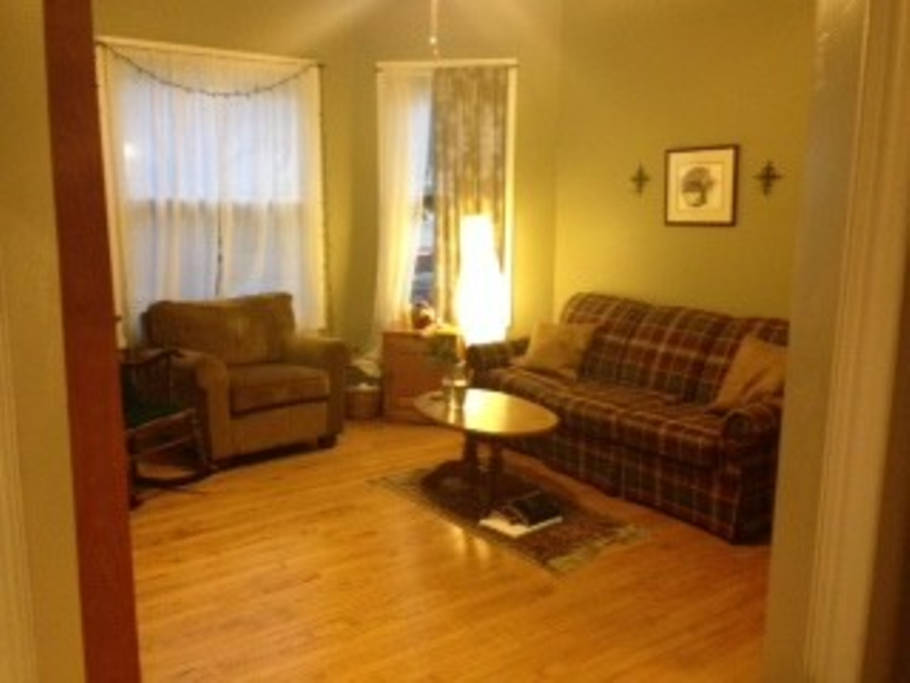
\includegraphics[width=0.5\columnwidth ]{pics/low/915372.jpg}
%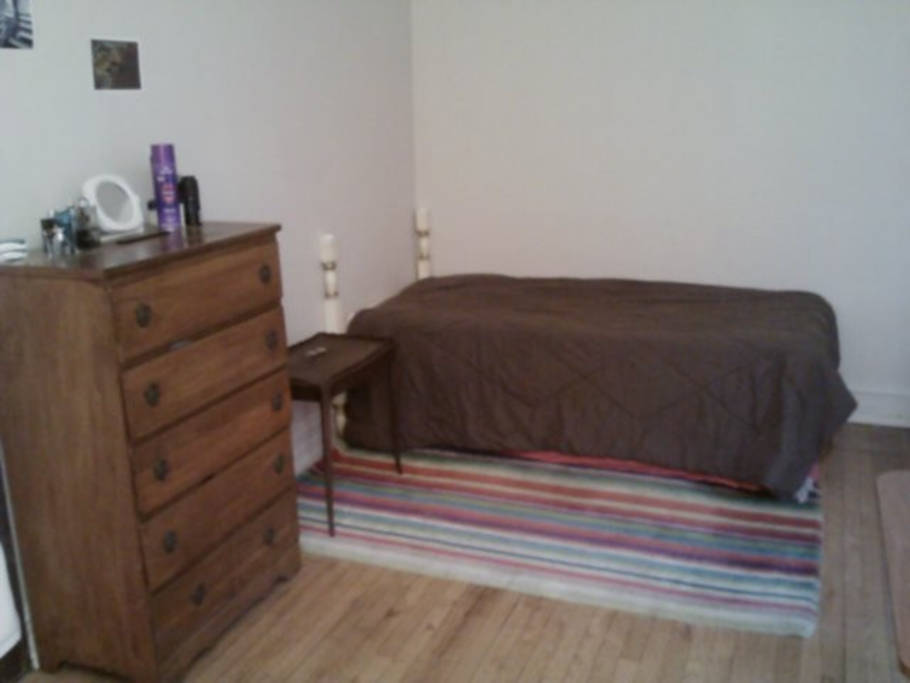
\includegraphics[width=0.5\columnwidth ]{pics/low/13892310.jpg}
%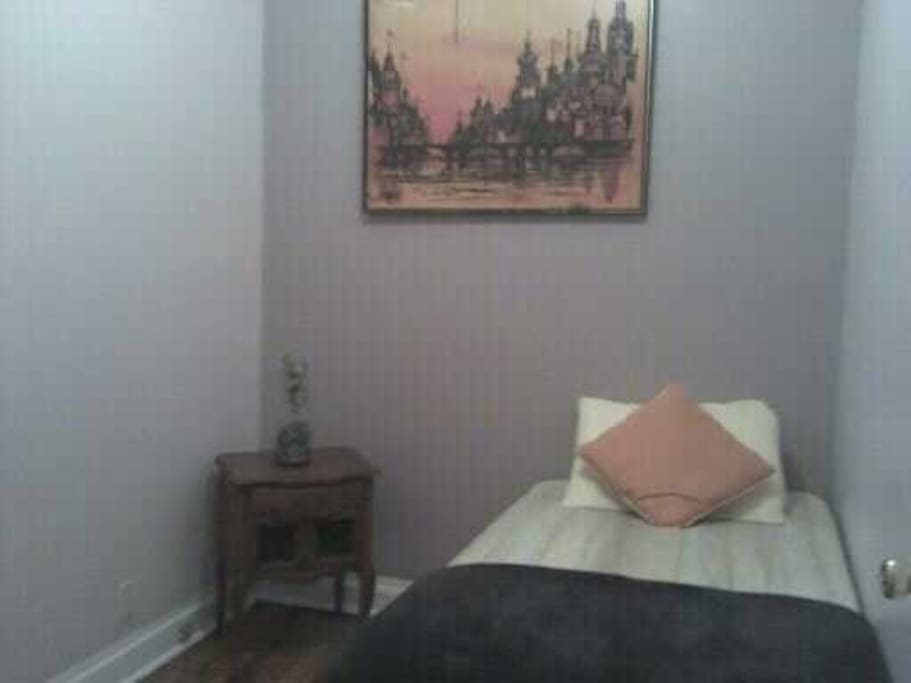
\includegraphics[width=0.5\columnwidth ]{pics/low/10227627.jpg}
%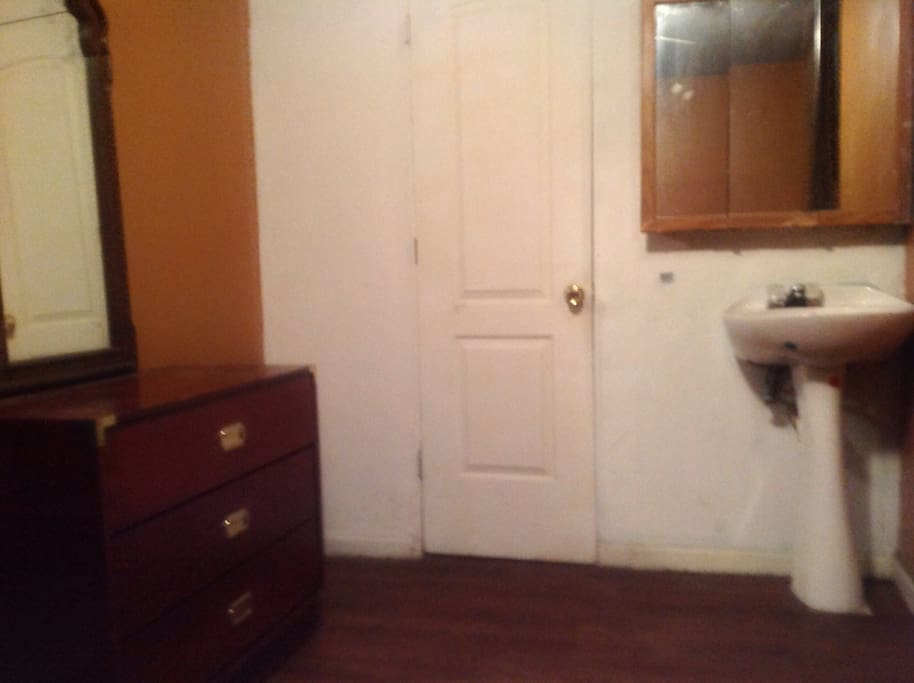
\includegraphics[width=0.5\columnwidth ]{pics/low/3751869.jpg}
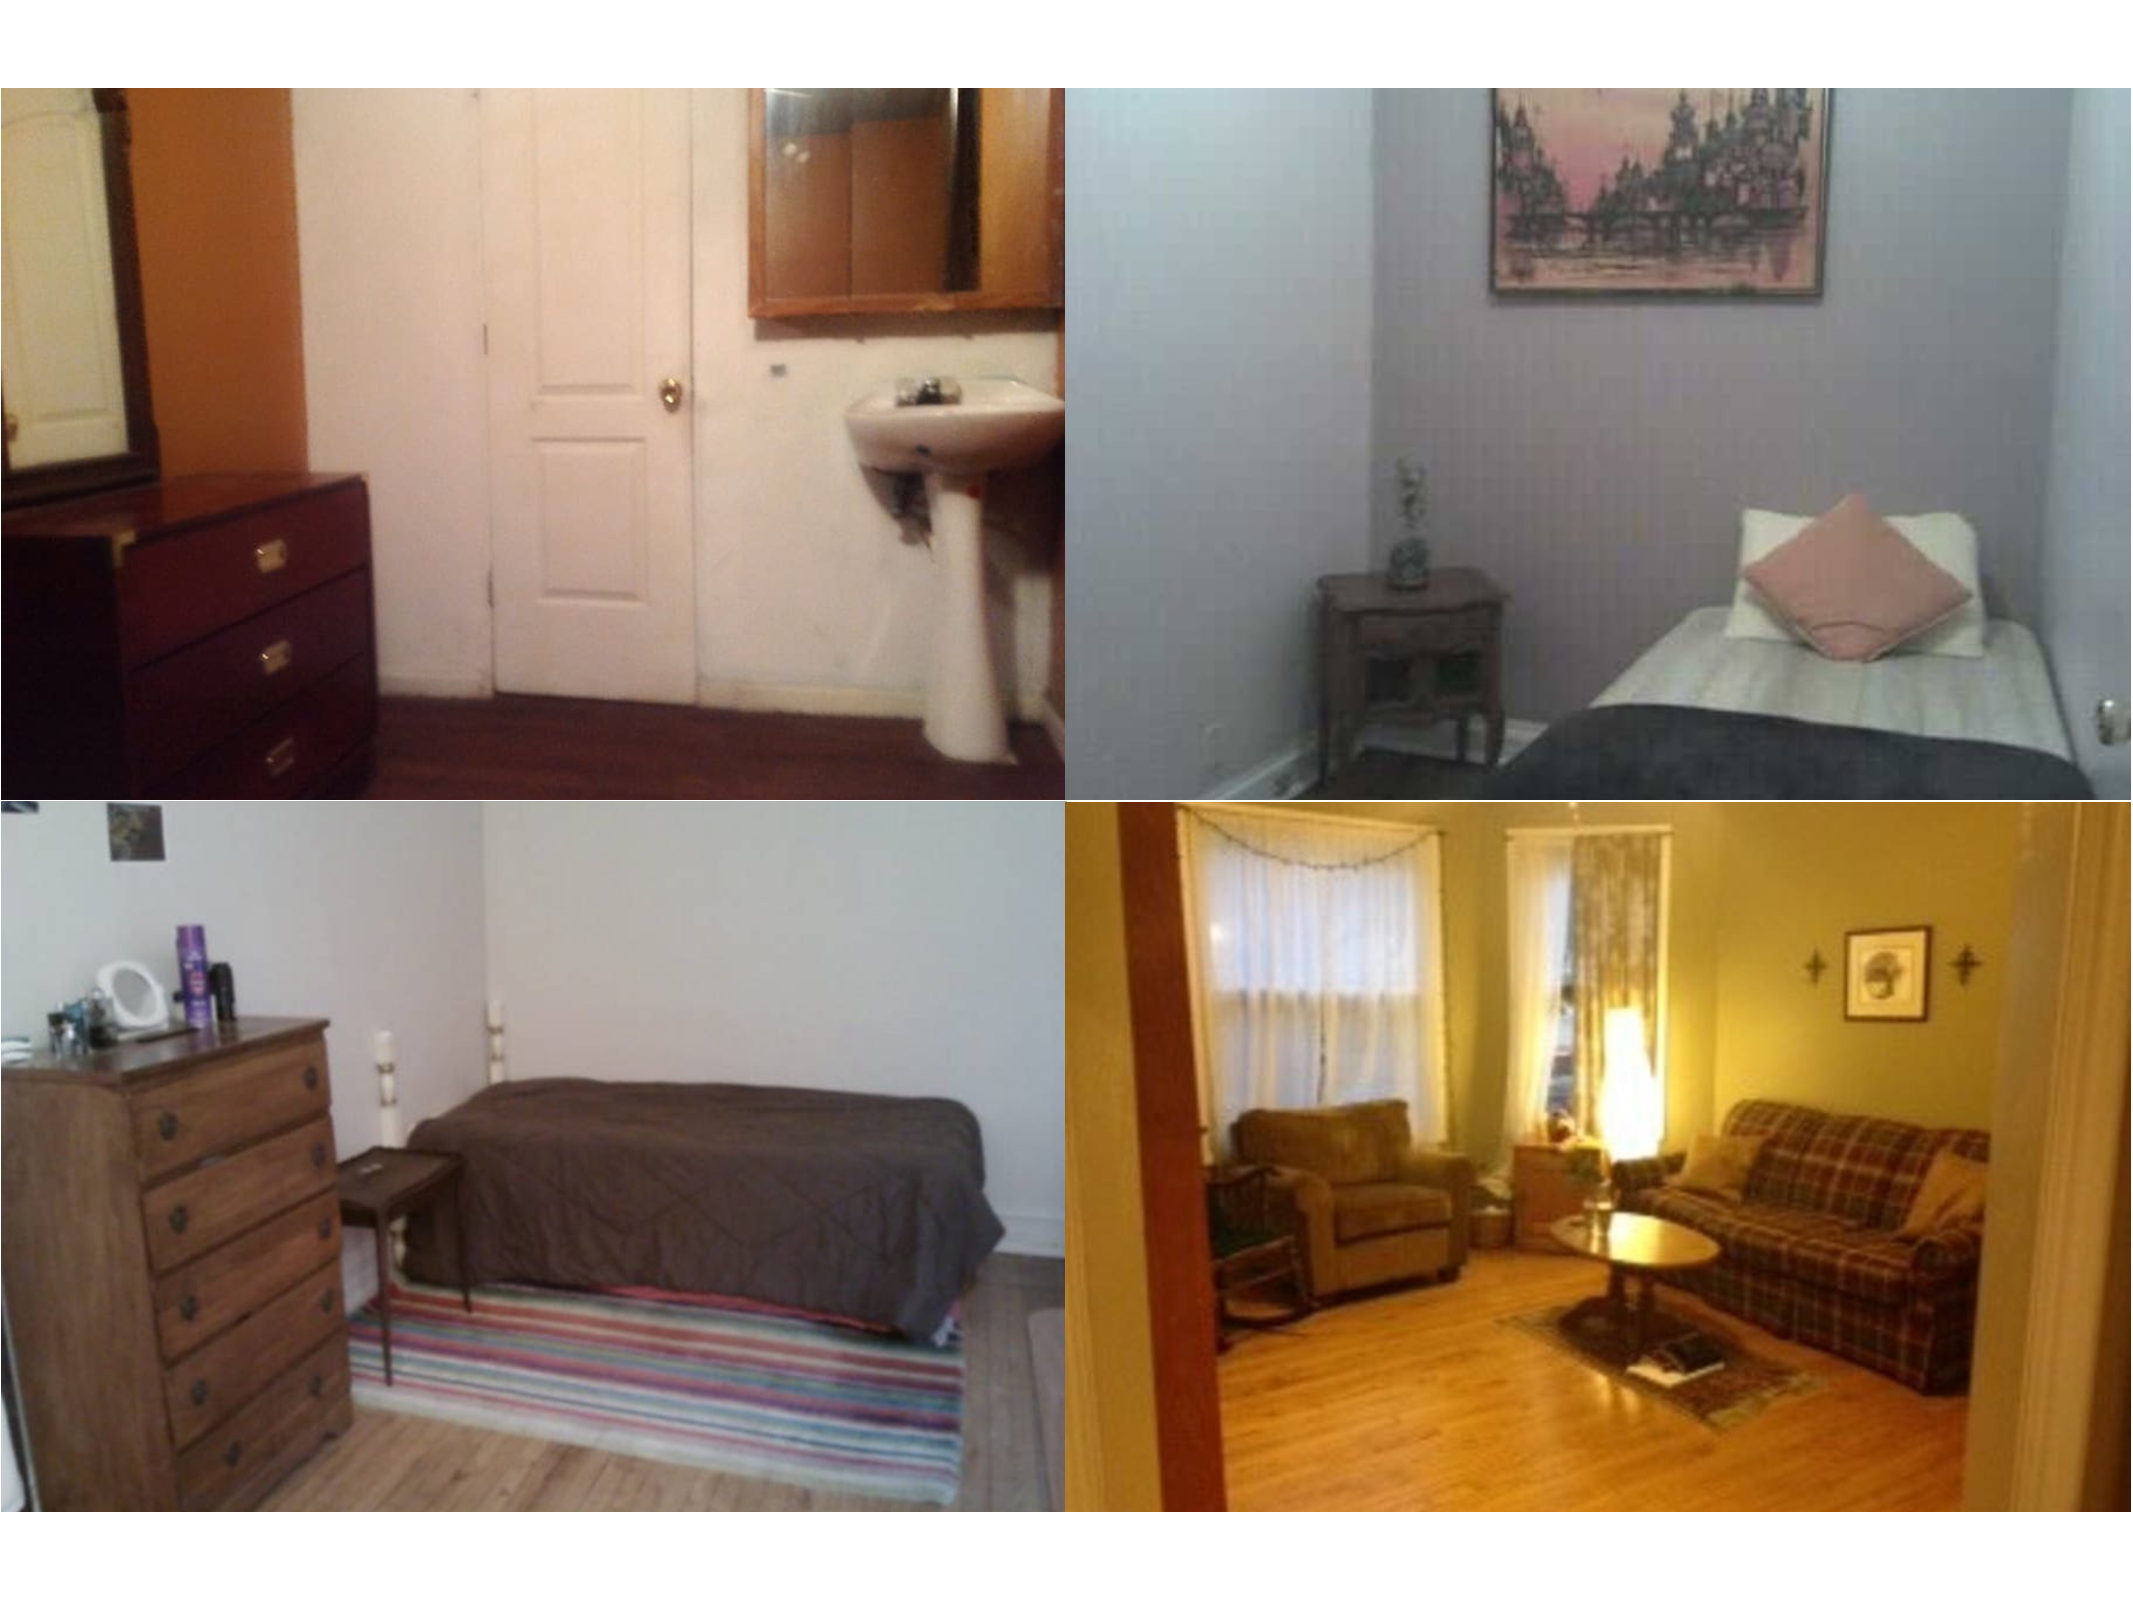
\includegraphics[width=0.4\columnwidth]{pics/low.pdf}
%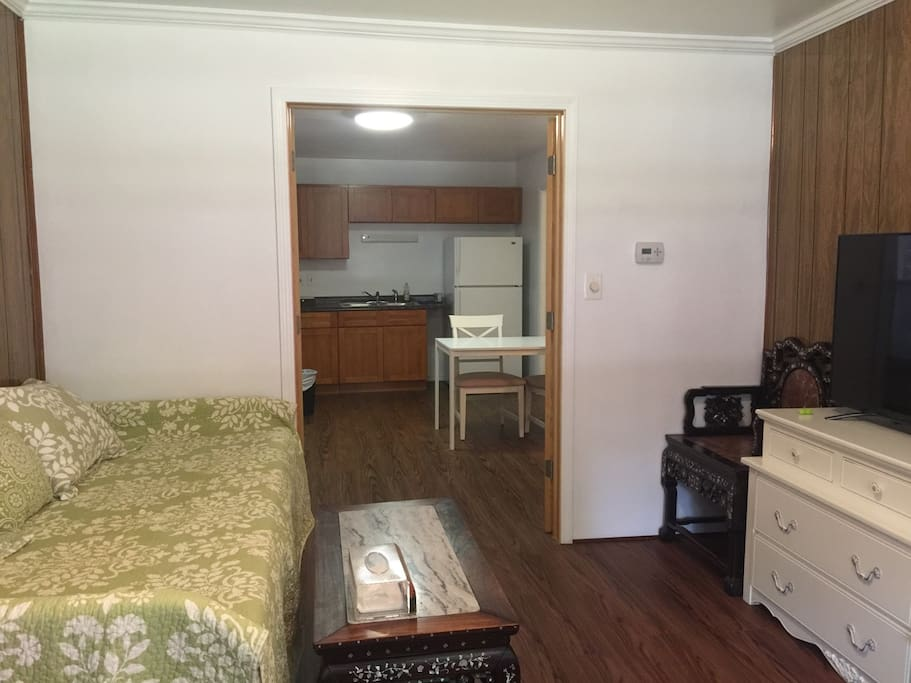
\includegraphics[scale=0.1]{pics/medium/13890897.jpg}
%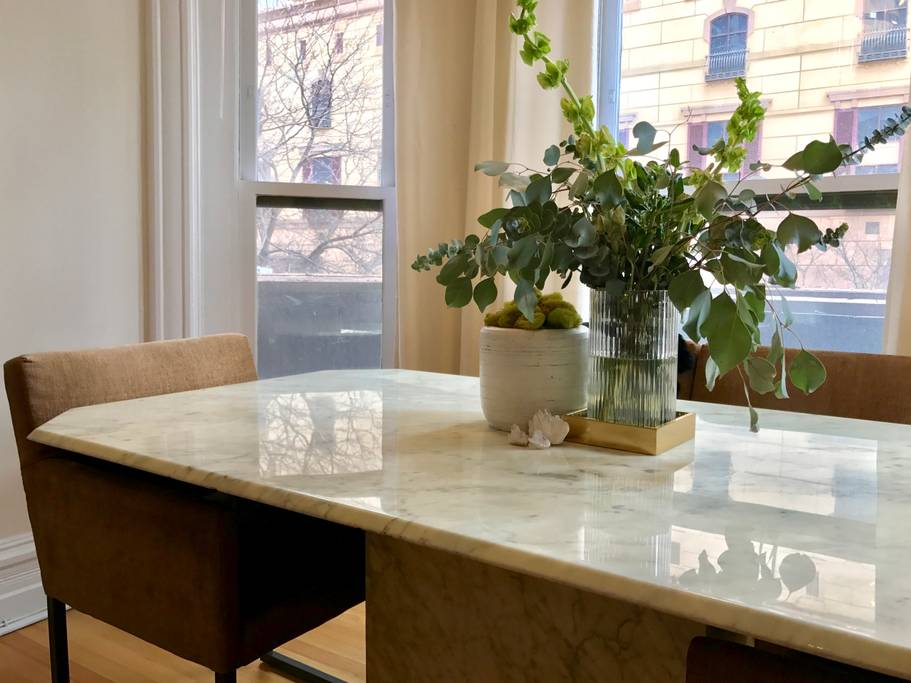
\includegraphics[scale=0.1]{pics/medium/17909111.jpg}
%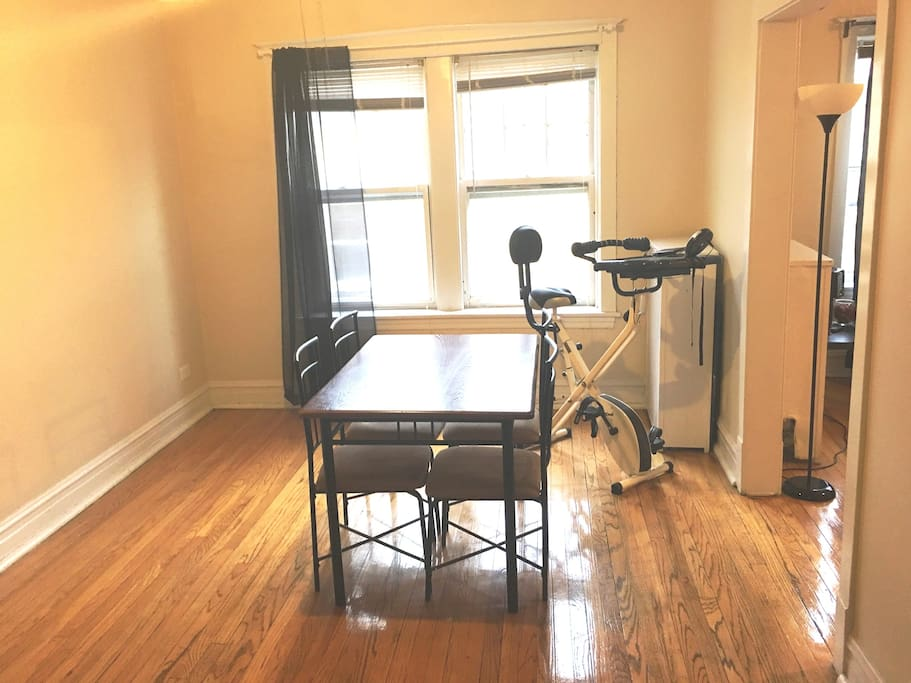
\includegraphics[scale=0.1]{pics/medium/18157129.jpg}
%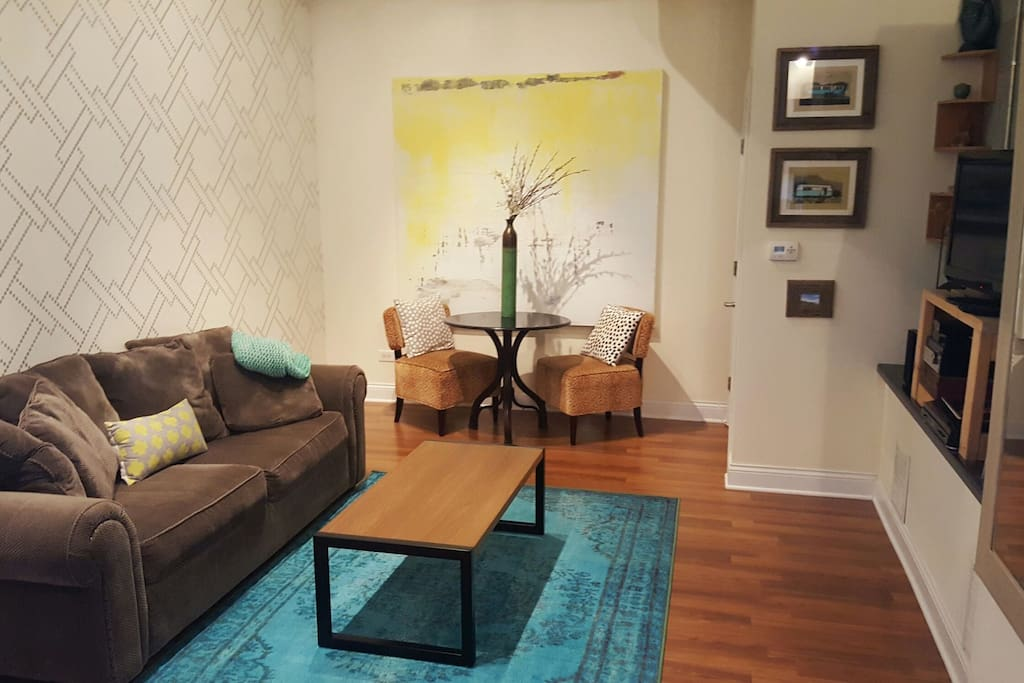
\includegraphics[scale=0.1]{pics/medium/13149571.jpg}
%\\
%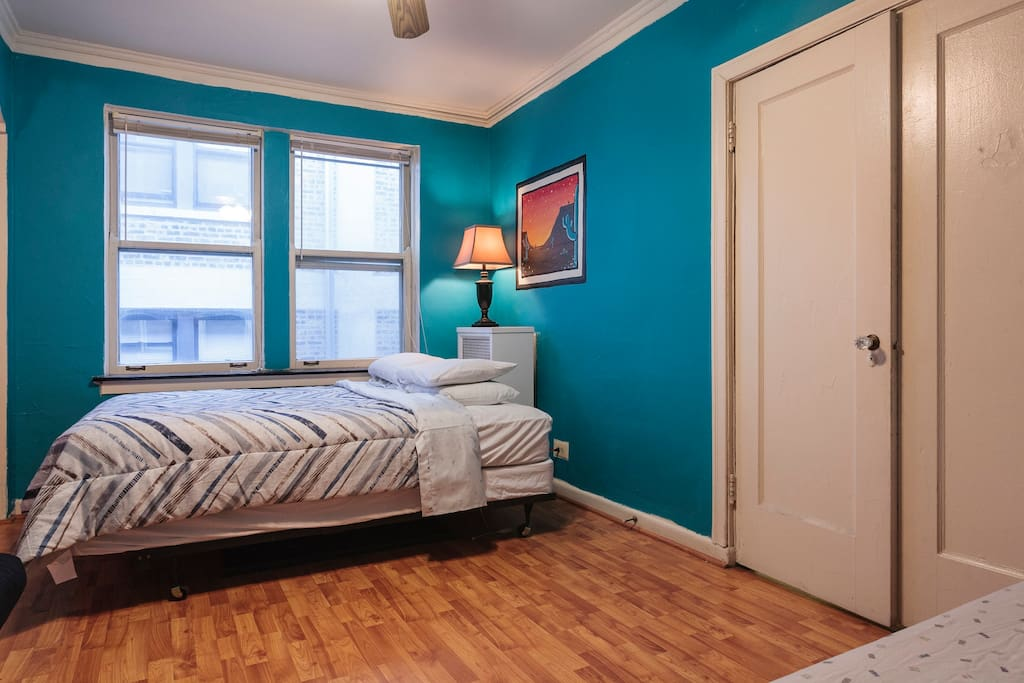
\includegraphics[width=0.5\columnwidth]{pics/high/8207547.jpg}
%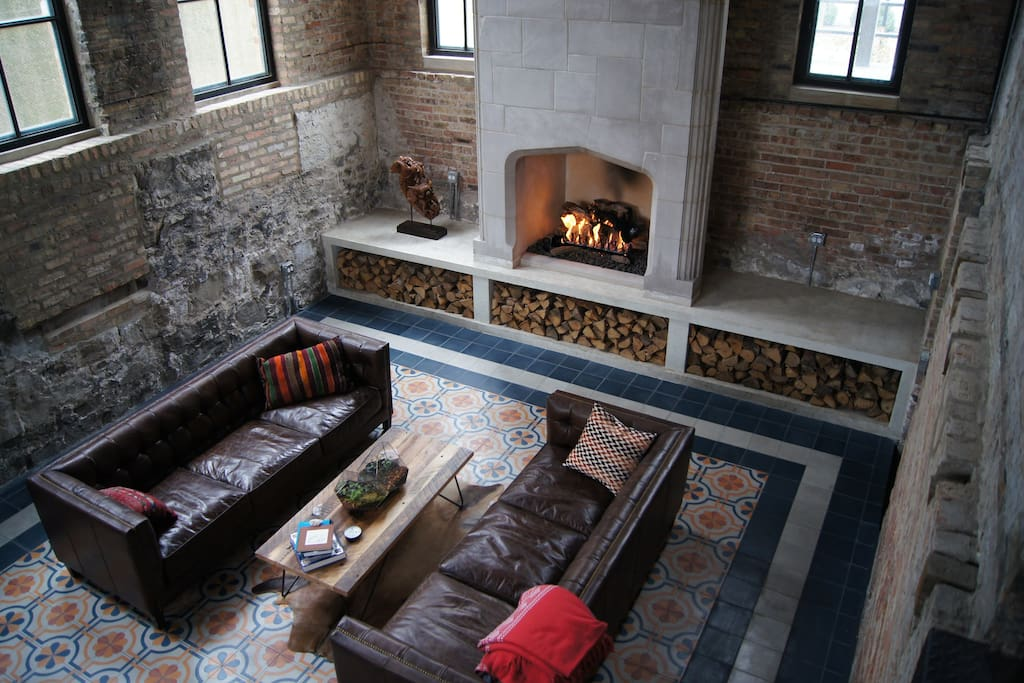
\includegraphics[width=0.5\columnwidth]{pics/high/16812497.jpg}
%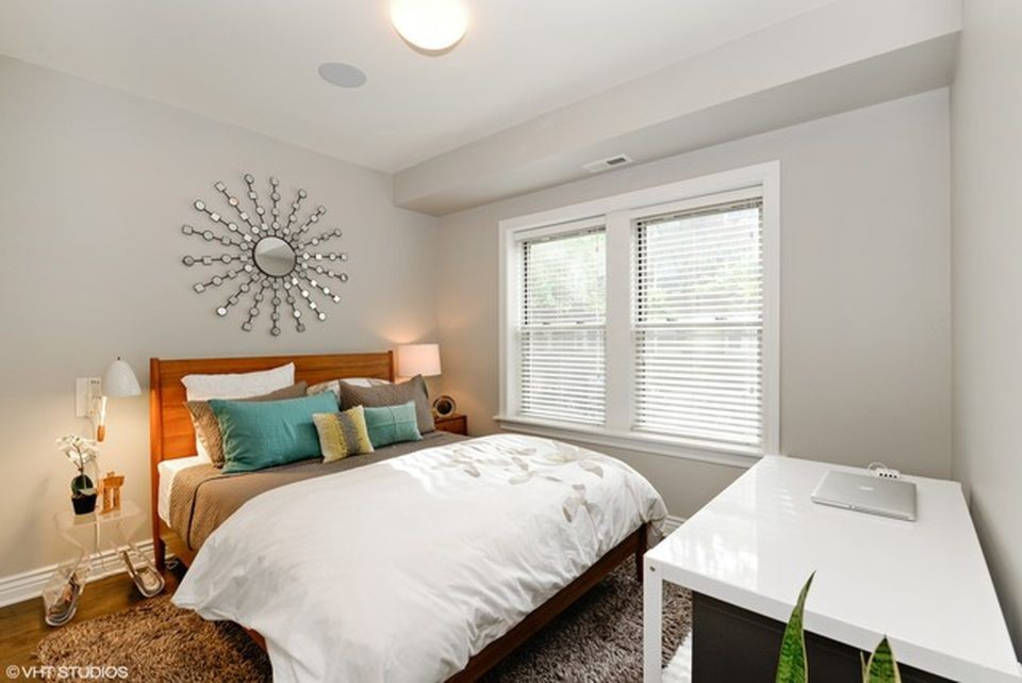
\includegraphics[width=0.5\columnwidth]{pics/high/17253265.jpg}
%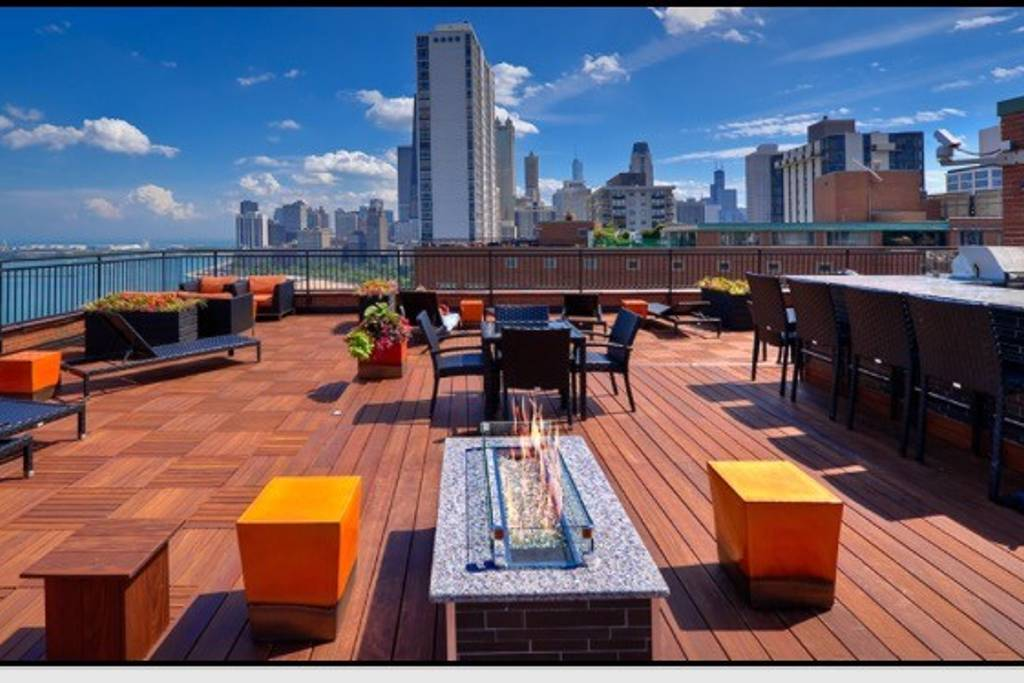
\includegraphics[width=0.5\columnwidth]{pics/high/18061514.jpg}
\includegraphics[width=0.4\columnwidth]{pics/high.pdf}
\caption{Example of images with  low and high  aesthetic score calculated based on ILGNet~\cite{ilgnet}.}
\label{fig:aesimages}
\end{center}
\end{figure*}


\subsection{Airbnb Dataset}
\ab \ does not provide an API to access their dataset, therefore for our study we relied on external sources that collected listings. More specifically we used the listings of Chicago that were last  scraped in May 2017 by InsideAirbnb\footnote{http://insideairbnb.com/ last retrieved on Jan 2018 }; an independent, non-commercial website that provides set of tools and data that allows everyone to explore how Airbnb is really being used in cities around the world.

This dataset includes the all the listed properties in the Chicago region along with the  following  information about the hosts and property. Specifically we consider the following attributes: 

\begin{itemize}
\item Host:  name, photo URL, the date the host joined \ab, the number of listings they have, whether they are a super-host\footnote{Super-hosts in the \ab \ platform are those who hosted at least 10 trips, maintaining at least a 90\%  response rate and received  a 5-star for  at least 80\% of the time they have been reviewed.} or not and finally information on the number of reviews and a user generated scores broken down by communication, interaction and location.

\item{Property}:  photo URL,  price, type of the property (Private/Shared room or Entire Place) as well as  latitude and longitude. 

\end{itemize}

The dataset includes 5200 listings of which 60\% are for renting the entire home/apartment. Moreover, these listings are offered by 3500 uniques hosts. Indeed, the dataset in hand presents that 48\% of the listings are by hosts who offer more than one property, with some of the hosts offering up to one hundred different rooms and houses. These hosts often present lodging business or state agents who use \ab \ platform to rent their various properties.  In this paper as we are interested to uncover social inequality on the individual scale, we filter out all those hosts (and their listings) that have more than one property presented in Chicago during the same time period that the dataset was scrapped. The resulting dataset includes 2700 listings by same number of hosts. 
 
 %final set of features we use
%properties of the dataset 
 
\subsection{American Community Survey}
In addition to the \ab \ dataset we also required information about the socio-economic status of the hosts. We gathered median household income data (Figure~\ref{fig:census}) from the 2016  American Community Survey (ACS). This metric is known as an indicator of socioeconomic status~\cite{li2013spatial}. It is also been shown to be highly correlated with education and unemployment. We also collected the number of household units and the population of \aam, White and Asian households per tract from the ACS (Figure~\ref{fig:census}) .  Throughout our analysis, we chose the level of the census tracts \footnote{Census tracts are geographic areas defined by the U.S. census and generally have a population size between 1,200 and 8,000 people, with an optimum size of 4,000 people.} in terms of granularity as it provides us with a relatively small geographical unit.  Furthermore it allows us to  keep consistent and thus making our findings comparable with other  geographical studies~\cite{Thebault-Spieker17} on the sharing economy.  By combining this dataset with the host demographics identified through photo identification, we calculate an ethnical discrepancy metric for each census tracts as we will describe in the next section. 
 
  
\begin{figure*}[!h]
\begin{center}
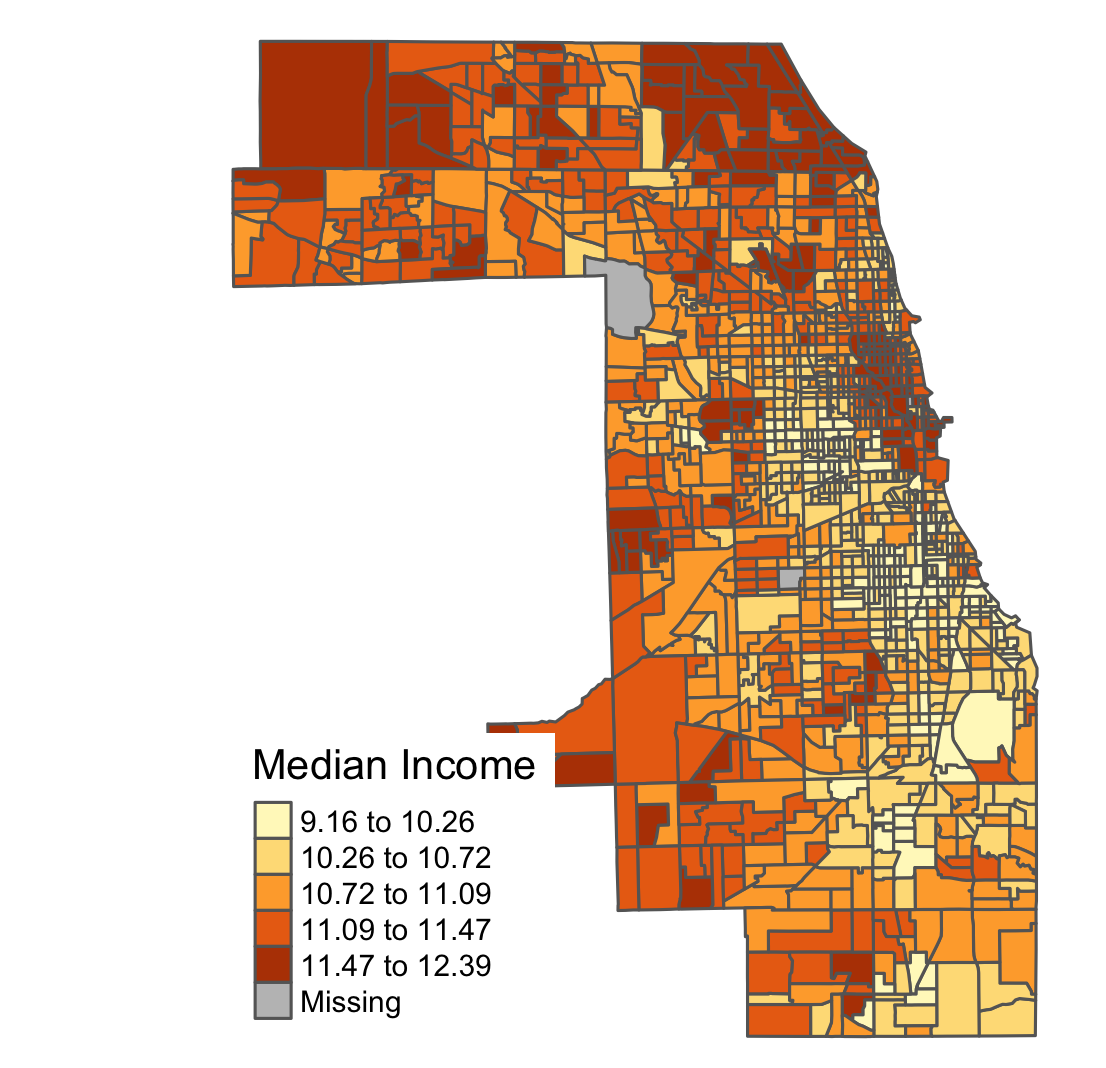
\includegraphics[scale=0.13]{pics/income.png}
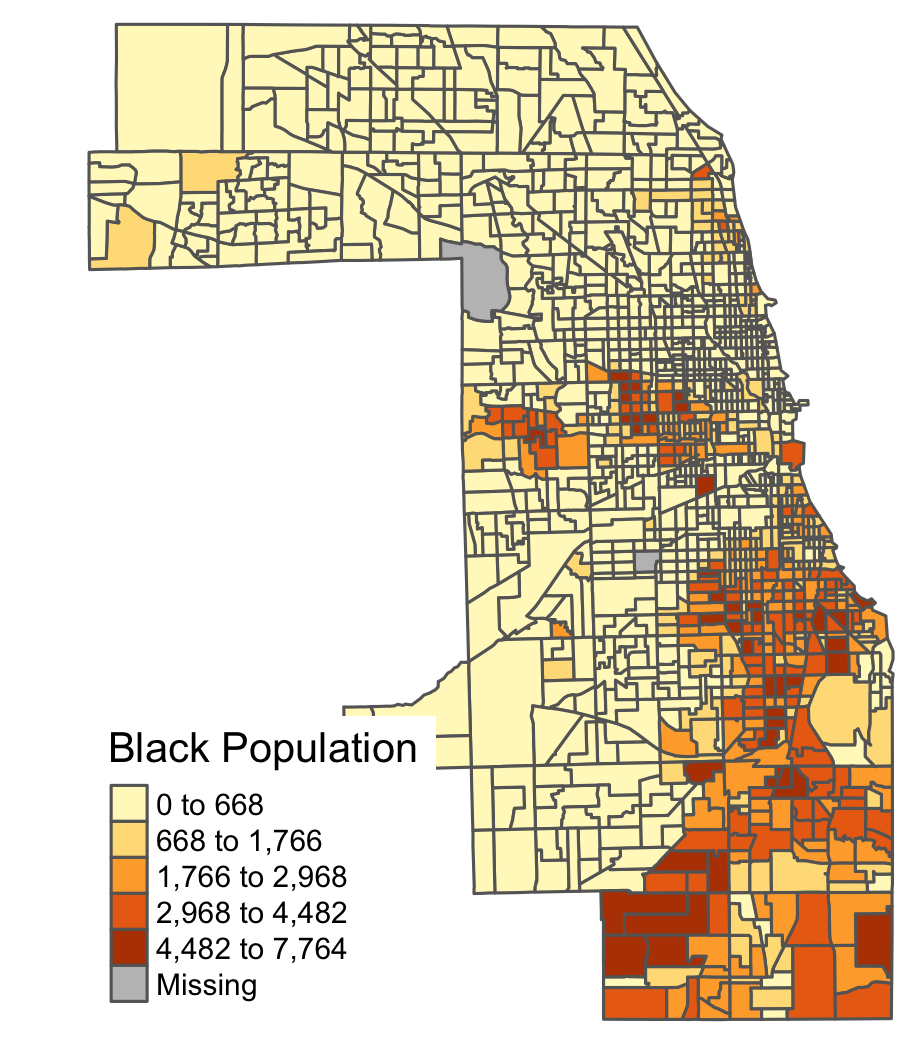
\includegraphics[scale=0.13]{pics/black-census.png}
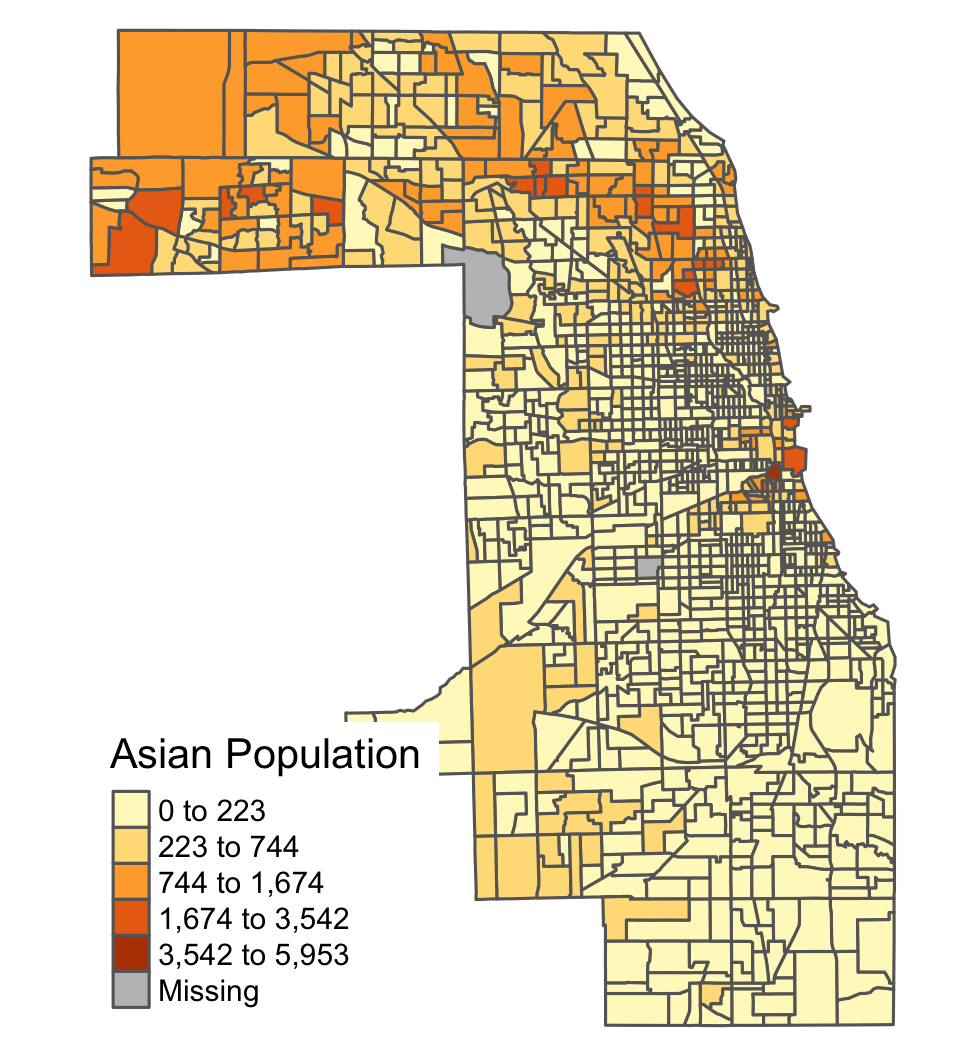
\includegraphics[scale=0.13]{pics/asian-census.png}

\caption{Median household income (in log scale), geographical distribution of \aam \ population, and geographical distribution of Asian population in the greater Chicago area based on the  2016  American Community Survey Data.}
\label{fig:census}
\end{center}
\end{figure*}

\subsection{Demographic Analysis}

\ab \ does not provide any demographic information regarding the host. Therefore we required a technique to automatically detect gender, age and ethnicity. There are currently two possible techniques to do so: one is to process the textual content such as name and the description of the host, to detect the demographics. However this method is known to be error prone as hosts can present themselves with nicknames or arbitrary usernames, and the language used in providing the description of themselves is likely to follow a formal template, making it hard to detect age and the language skill of the writer. An alternative method is to extract demographic data using the host profile picture.  Relying on the latter choice we crawled the host profile photos from the \ab \ website and used the Face++\footnote{Face++. http://en.faceplusplus.com/, 2013.} API to process them. Face++ provides a set of  powerful, and cross-platform vision services which enable us to detect age, gender and race through facial recognition techniques. The API does not provide an estimation of accuracy, however studies that used this API for the similar identification purpose such as~\cite{bakhshi2014faces} have reported of 97\% accuracy when validated against crowd-sourced Mechanical Turk platforms.

\subsection{Aesthetic Analysis}
In order to quantify the aesthetic level of images that hosts present in \ab \ we used advances in deep convolutional neural
network (DCNN) that capture both global and local features.  Local characteristics include noise, blur and contrast while global characteristics include composition features such as rule of thirds, foreground/background separation, depth of field etc. 
In particular we used ILGNet~\cite{ilgnet} a DCNN based algorithm which  introduces the inception module that connects two intermediate local layers to the last layer which extracts the global features for the output. Furthermore this algorithm is based on a pre-trained image classification CNN called GoogLeNet on the ImageNet dataset and  fine tuned on the Aesthetic Visual Analysis (AVA), is a large dataset formed by more than 250 thousands of images~\cite{murray2012ava}. Figure~\ref{fig:aesimages} shows an example of the photos that were classified with a high and low aesthetic score.



\section{Results}

In this section, we report the results of our work based on five complementary sets of analyses: 

\begin{itemize}
\item The geographical distribution of the listings.
\item The demographic composition of the hosts.
\item The services offered by the hosts.
\item The aesthetic presentation of the listings.
\item The pricing and ratings that hosts receive.
\end{itemize}


\subsection{Geographical distribution of \ab \ listings }

\begin{figure*}[!h]
\begin{center}
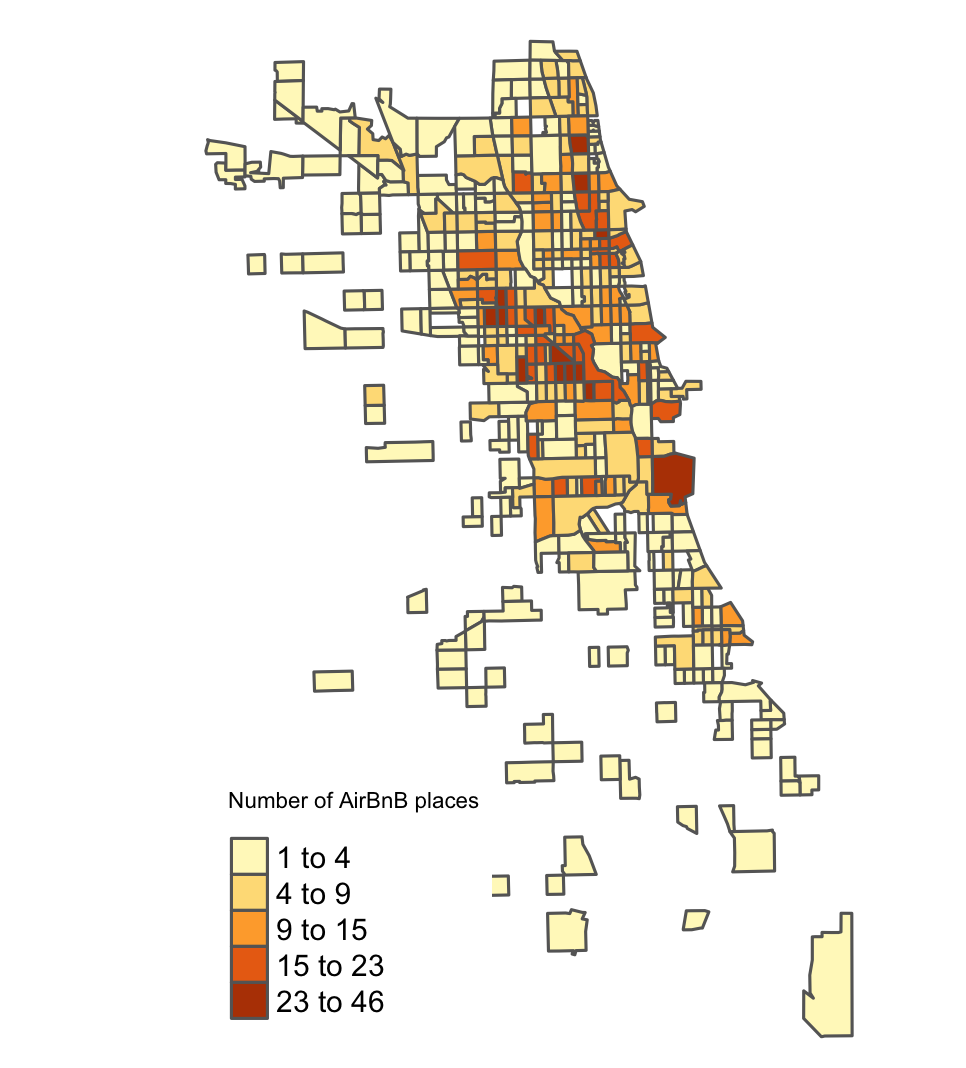
\includegraphics[scale=0.20]{pics/listings.png}
%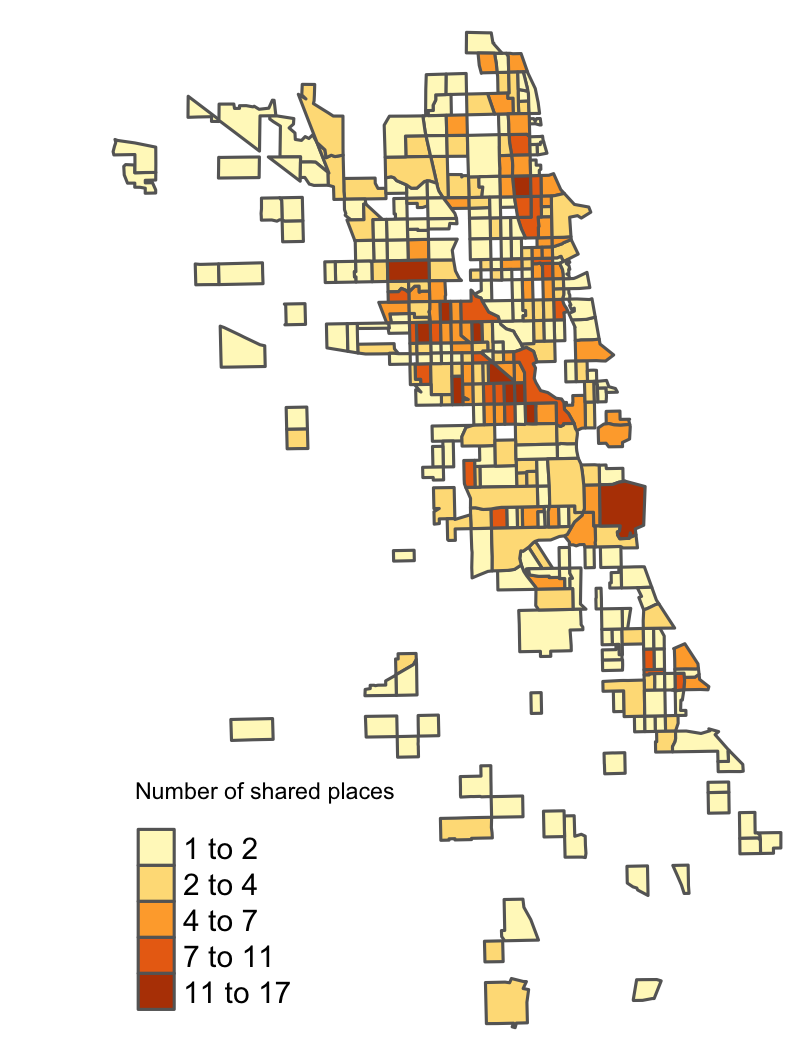
\includegraphics[scale=0.20]{pics/shared.png}
\caption{Geographical Distribution of AirBnB Listings (non-shared and shared).}
\label{fig:alllistings}
\end{center}
\end{figure*}

\begin{table}[htp] 
\begin{center}
\begin{tabular}{c|c|c}
& Median  Income & Household units \\
\hline
\hline
Number of Listings &  0.29 *** & 0.37 ***\\
%\hline
%Number of Shared &  0.20 *** & 0.25 ***\\
\hline
Number of Super-hosts &  0.24 ***& 0.18 ***\\
\hline
\end{tabular}
\end{center}
\caption{Pearson's correlation Coefficient and p-value. *** indicates p-value $\leqslant$ 0.001}
\label{tab:pre}
\end{table}%



%The examination of the geographical distribution of \ab \ listings in Figure~\ref{fig:alllistings}, presents the placements of all \ab \  listings as well as the subset of listings that were shared listings.
The examination of the geographical distribution of \ab \ listings in Figure~\ref{fig:alllistings}, presents the placements of all \ab \  listings.

As expected, most of listings are placed in the downtown area.
Furthermore, there are more listings in the richer northern suburbs of Chicago as opposed to the poorer and more racially diverse southern suburbs.

Pearson's correlation between the number of \ab \ listings and the census variables obtained from the American Community Survey (Table~\ref{tab:pre}), confirms that most properties are in richer and more dense areas, it also suggests that the super-host properties are placed in tracts with higher median household income.

%These results confirm previous findings in the literature, however this is at a high, aggregate level and does not provide insights into who the actual hosts are, their demographics and their offering on the \ab \ platform.


\subsection{Demographic analysis of the hosts}

Using the facial-recognition capabilities of Face++, we provide an overview of the demographic makeup of \ab \ hosts using an analysis of host profile pictures. Face++ predicts age, gender and ethnic background.

Face++ identified more than one person in 30\% of the host pictures.
These hosts and their listings were removed from our analysis, since  their identity could not be garanteed.

In the remaining 1700 hosts and their listings, Face++ reported, 47\% female 53\% male, 13\% Asian, 11\% African-American and 76\% White\footnote{Note that Face++ does not identify hispanic as a separate ethnic classification.} (Table~\ref{tab:age}).

\begin{table*}[h]
    \centering
    { \tablesize
    \begin{tabular}{l c c @{ } l}
    \multicolumn{1}{c}{\emph{Race}} &\emph{Percentage}     & \emph{Age Distribution}        &\emph{Female - Male}\\
    \hline
    Asian                         &  13\%     & \myhist{asianage}                 & 53\%-47\% \\
    African-American         &   11\%       & \myhist{blackage}       &  43\%-57\%\\
    White                            &   76\% & \myhist{whiteage}              &  48\%-52\%\\
    \hline
    \end{tabular}}
\caption{Demographic properties of \ab \ Chicago hosts based on the analysis of their profile picture.  }
\label{tab:age}
\end{table*}

%In order to understand the relation between these demographic variables (age, race and gender) and how the hosts use the \ab \ platform,

The cross-correlation matrix of demographic variables where the Pearson's correlation p-value is less than 0.01 (Figure~\ref{fig:correlation}), shows, as expected, that the number of reviews and reviews per month are highly positively correlated and also correlated with a super-host status. There was a weak positive correlation between super-host status and both age and membership duration (\emph{host\_duration}).

Interestingly, there is a positive correlation between age and white ethnicity, indicating that older hosts are more likely to be white, and a weaker negative correlation with gender, indicating that older hosts are more likely to be male.

%No other correlation between the type of the property (whether it is an entire place or shared) and other variables. 

 
\begin{figure}[h]
\begin{center}
%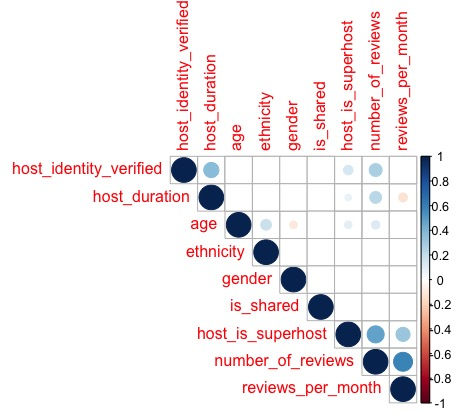
\includegraphics[width=\columnwidth]{pics/corplot.jpeg}
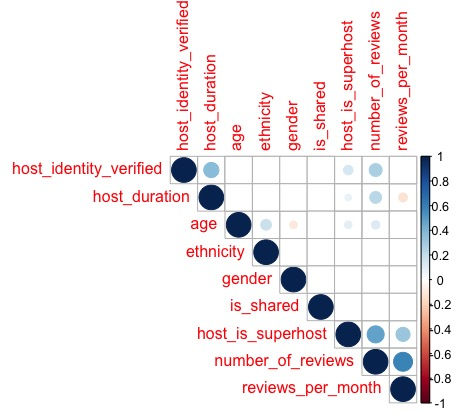
\includegraphics[scale=0.5]{pics/corplot.jpeg}
\caption{ Pearson cross-correlation matrix of the \ab \ platform features and the detected demographics where p-value significancy level is less than 0.01. Gender coded as female=1 and male=0 and ethnicity as white=1 and other=0. }
\label{fig:correlation}
\end{center}
\end{figure}



\subsection{Analysis of the properties offered }

Having examined the demographics of the \ab \ hosts for the dataset in hand, we now turn our focus to understanding what these hosts offer.   %Although the cross-correlation matrix did not support any correlation between the demographics variables and the type of the property (the entire property vs shared room)....<HERE> 

To this end, we calculate a residual metric which measures the discrepancy between the actual ethnicity ratio of the \ab \ hosts and the expected ratio based on the census population of these communities.

ratio of African-American/asian hosts in \ab \ 

We measure the actual ratio by dividing the number of African-American/Asian hosts by the total number of \ab \  hosts in each census tract.
We then calculate the residual by subtracting this measure from the ratio of  the census. The higher the value of the ethnicity residual the bigger is the discrepancy between the ethnical background of the residents and the \ab \  hosts.
 
Figure~\ref{fig:gap} presents area cartograms  of the ethnicity gap for African-American and Asian population in the greater Chicago area.

In this figure, the tracts are colored according to the level of over- or under-representation, with a green color representing the tract with extreme under-representation of the African-American (or Asian) hosts compared to the residential population.

To put these discrepancy values into context,  we calculated two linear regression models with the dependent variable as the discrepancy value and census variables as independent variables.

Table~\ref{tab:reg} presents the details of these models.

As it can be seen we observe a significant negative correlation with the median household income for the African-American discrepancy.

That is the poorer areas (those concentrated in southern part of Chicago) also exhibit higher under-representation in \ab.

This result indicates that those who could perhaps most benefit from the opportunities of micro-entrepreneurship are those who are not sufficiently represented in the system.  

\begin{figure*}[htbp]
\begin{center}
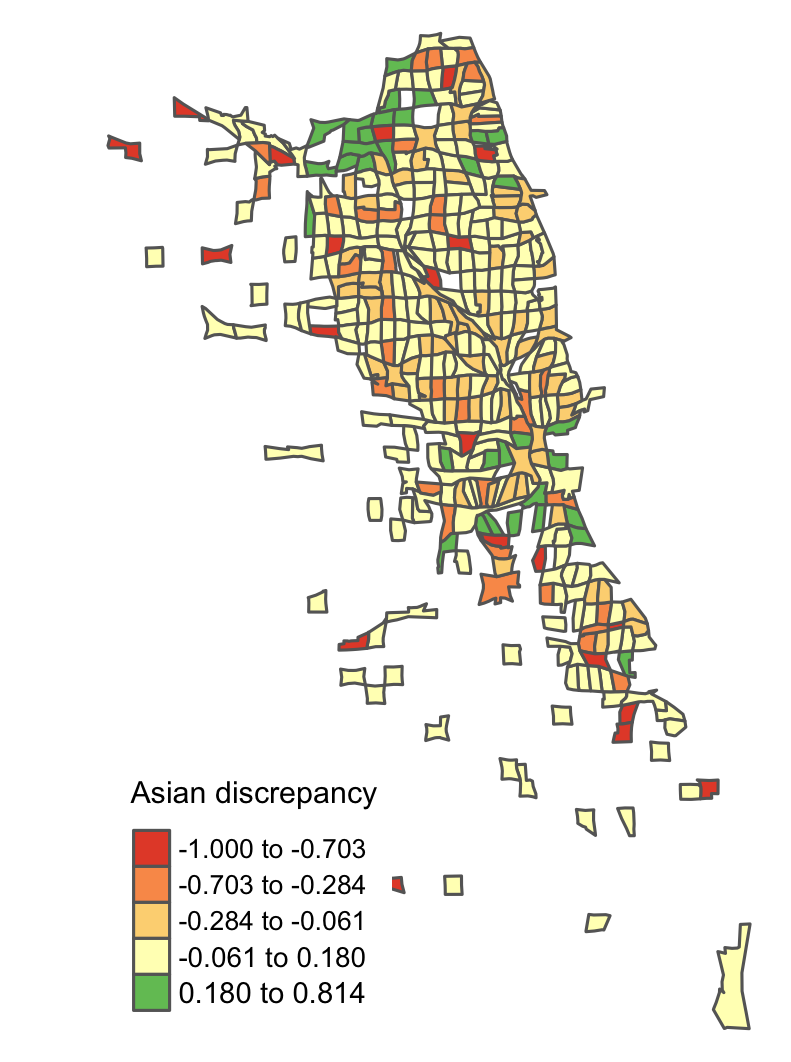
\includegraphics[scale=0.25]{pics/asian-gap.png}
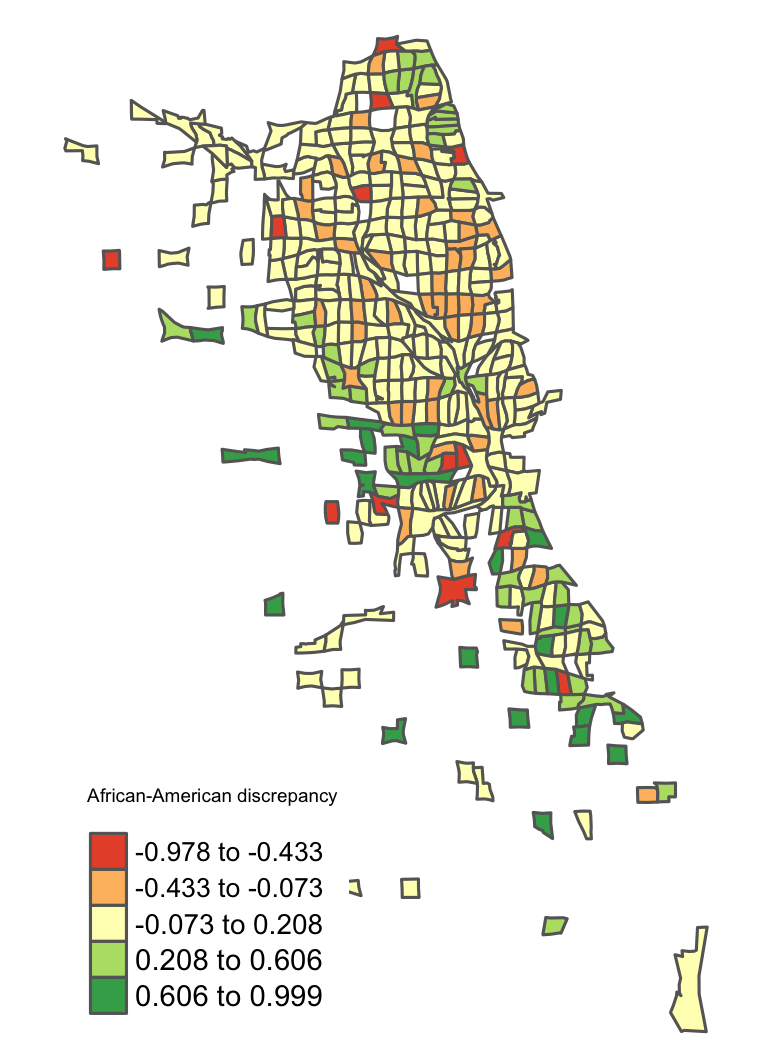
\includegraphics[scale=0.25]{pics/black-gap.png}

\caption{ An area cartograms based on the ethnicity gap where the green color (higher values) present areas in which there is the highest discrepancy between the ethnical background of the residents and the \ab \  hosts. }
\label{fig:gap}
\end{center}
\end{figure*}

 
   \begin{table}
        \centering

        \begin{tabular}{c|c c|c c}
%            \cline{2-5}
             & \multicolumn{2}{c}{African American } &  \multicolumn{2}{c}{Asian }\\
              \cline{2-5}
             & $\beta$ & p-value &  $\beta$ & p-value\\
           \hline
            \hline
              Median Income & -0.29 & *** & 0.00 &   \\
            No. Household & -0.07 & **  & 0.03 & . \\
            \hline
            \hline
            Adjusted R-squared    & \multicolumn{2}{c|}{ 0.224} &  \multicolumn{2}{c}{ 0.001}\\

        \end{tabular}
\caption{Regression analysis of the discrepancy value for African-American and asian communities in relation to the income and population data.  }
\label{tab:reg}
    \end{table}


\subsection{Aesthetic presentation of properties}
%here some stats on the scores. 
We now turn our attention to how the hosts present their properties on the \ab \ platform. Figure~\ref{fig:aes} presents the frequency distribution of the aesthetic scores of all the images. As it can be seen the distribution is skewed toward higher scores, demonstrating that most of the images in our dataset are both of good quality (local features), and well composed (global features). Indeed, we manually checked the images that had a very low aesthetic score (falling below the first interquartile range~-- IQR) and found that most of those images suffer from low local properties and in many cases are blurred. 

\begin{figure}[!h]
\begin{center}
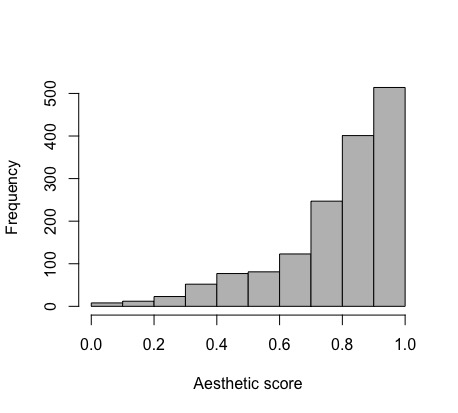
\includegraphics[scale=0.3]{pics/Hist-aes.jpeg}
\caption{The frequency distribution of the aesthetic scores of the main property photos. }
\label{fig:aes}
\end{center}
\end{figure}

Figure~\ref{fig:score} presents the choropleth map of the median aesthetic scores for each tract. We observe a weak positive correlation (r=0.14, p-value=0.005) between the median household income and the median aesthetic scores of the images, suggesting that hosts in the poorer neighborhoods do not present listings as well as others, perhaps due to socio-technical challenges. 

\begin{figure}[htbp]
\begin{center}
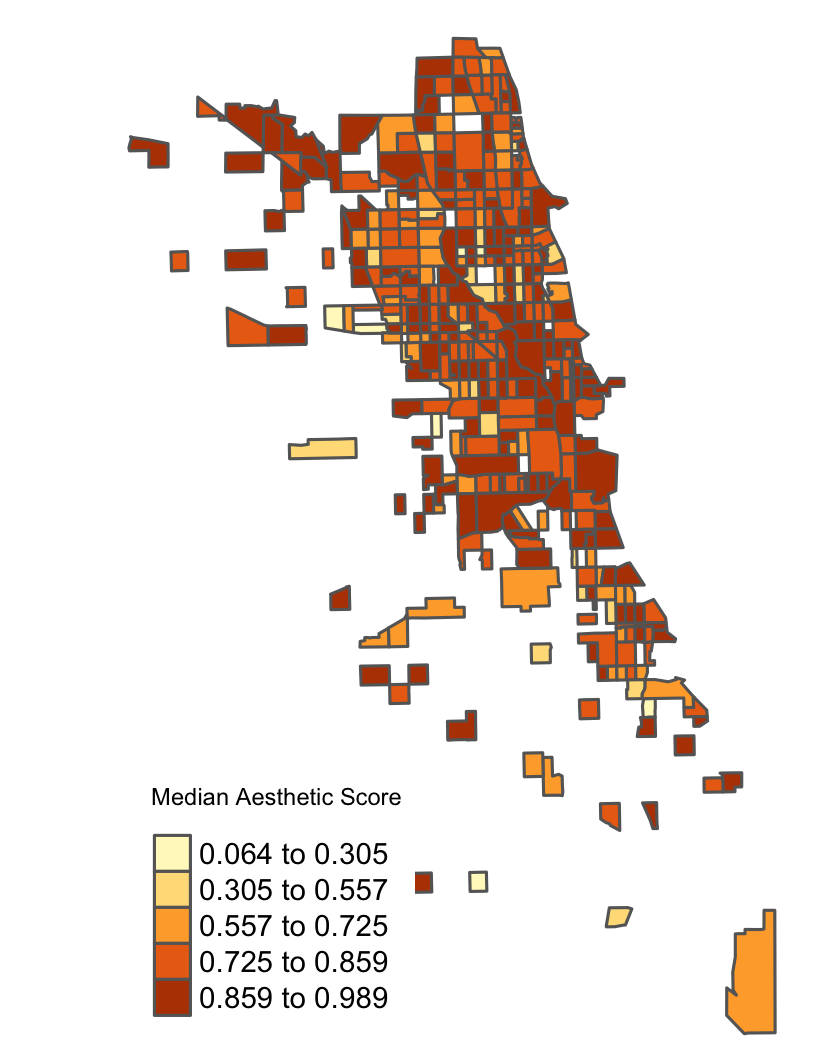
\includegraphics[scale=0.2]{pics/score.png}
\caption{The choropleth map of the median aesthetic scores. The lower shades present the areas with lower median aesthetic score. }
\label{fig:score}
\end{center}
\end{figure}


%We then conducted a  Welch Two Sample  t-test to compare the aesthetic scores between the hosts who had a property in the richest neighborhoods (where median income is higher than the third IQ) and those in the poorest neighborhoods  (where median income is less than the first IQ). The result of this analysis suggests that there is no significant difference between the two groups. That is being a host in a poorer neighborhood does not directly indicate poor quality of presentation on the platform. 


We then incorporate demographic of the hosts and conduct a series of  Welch Two Sample  t-tests  to compare the aesthetic scores between different i) female vs male ii) African-American vs white iii) asian vs white iv) super-hosts vs non super-hosts. We find no significant difference between the aesthetic scores of different genders. However, we find a significant difference in the aesthetic scores for the African-American (mean=0.75, sd=0.18) and White(mean=0.79, sd=0.18) hosts, with t(242)=-1.85 and p-value=0.03.  This gap widens even more (t(124)= - 2.31, p-value=0.01) when we compare the aesthetic scores for the African-American(mean=0.74, sd=0.18) and White (mean=0.8, sd=0.18) hosts in the neighborhoods where the median household income is in the first IQ (i.e., the poorest) and diminishes for the richer neighborhoods (with median income larger than the third IQ). Similar results were observed in comparing the aesthetic score of the Asian and White hosts.   Finally we find a significant difference (t(622)=2.09,p-value=0.01) between the aesthetic scores of super-hosts(mean=0.8, sd=0.17) compared to non super-hosts(mean=0.77, sd=0.19). We  do not observe any correlation between the aesthetic score of the images and the age of the host or the price of the property.  In summary, and complementing the prior section, it is primarily minorities from poorer neighborhoods that suffer from missteps in presenting their offerings.

%what is the relation between score and reviews 

Finally, we are interested in examining whether the aesthetic score actually has any impact on the host's success on the platform.
We use for this purpose the number of reviews per month as a proxy for demand and so an indicator of how successful a host is in renting out their property. We used reviews instead of ratings as an indicator of success because previous research has shown that  ratings are generally inflated and not very accurate~\cite{zervas2015first}. Furthermore Fradkin et al. have shown that more than  70\% of the times  people leave reviews after staying at a place~\cite{fradkin2015bias}.  As the popularity of a rental place is first and foremost dictated by its location, we calculate the median aesthetic scores and the median reviews per month for each census tract. We find a positive correlation of r=0.16 (p<0.001) between these two variables, indicating that the better the quality of the images, the higher the likelihood of the place being rented.   

A possible interpretation of these results is that hosts from a minority group and a lower socioeconomic background are those who require internal policies from \ab \ to assist them in presenting and offering their property on the platform. We discuss this implication in details in the next section.  


\subsection{Potential earnings from the platform}

%here 

Finally, we investigate whether there is any indication of social inequality when it comes to how the hosts of different background are treated, and how they price their listings. More specifically, we analyze social inequality in two ways:  i) what price do hosts from different  gender and ethnical backgrounds ask for; ii) whether the demographics of the host or their super-host status play a part in the ratings they receive from their guests.

Logically, both price and ratings are highly influenced by the type of property (number of rooms) and experience (e.g., amenities that are available on the site such as Wi-Fi or a hot tub) that is offered to the guests. To control for this dimension we conduct our analysis only for single private room places in \ab. %We also control for the location demand by computing median of the desired variables in each tract. We describe each analysis next:

Starting with pricing, for each tract we compute the average price based on all the private room properties that fall within that tract. We then compute a metric referred to as the \emph{price residual} by dividing the price of each listing by the average private room price for that tract. A value of less that one for this metric would indicate that the host is under-selling their property compared to the average room in the same area. We then compute a multiple linear regression model with the price residual as the dependent variable  and age, gender,  race and the super-host status as the independent variables. The model suggests a negative association between the \aam \ ethnicity and the price residual. A one-unit increase on the listings by \aam hosts predicts a decrease  of 0.12  in the  price residual  (se = 0.05); this decrease is significant, t(643 ) = -2.141 , p $<$ 0.01.  This result suggests that African-American AirBnB users earn 12\% less rent than other hosts for the same type of house in the same type of location. We do not find any  associations between the rest of the independent variables, which also suggests that the super-hosts do not over/under-sell their property. 


To understand whether there is a racial bias in how the hosts are rated, we use the location rating of the hosts as it corresponds to the satisfaction of the  guests with the location of the property and is meant to be independent of other factors such as amenities available at the property.  Similar to the previous metric we calculate the \emph{location rating residual} which corresponds to the    location rating of a listing divided by the average location rating of the tract.  A value of less that one for this metric indicates that the hosts are unfairly scored down. We then compute a multiple linear regression model with the location rating residual as the dependent variable  and age, gender,  race and the super-host status as  the independent variables. The model suggests a positive association between the super-host status and the location rating residual. That is a one-unit in the number of super-hosts   predicts a slight increase  of 0.01  in the  location rating residual  (se = 0.003); this increase is significant, t(643 ) = -2.755 , p $<$ 0.01.    We do not find any  associations between the rest of the independent variables, which also suggests that based on our dataset we do not observe that hosts of different demographic and racial background get scored down systematically. However, our result suggests that the super-hosts have an slight advantage and they are scored higher in terms of location rating compared to others hosting the same neighborhood.  


%super hosts and eldely get slightly higher rating for the location


\section{Discussion}
In this paper we studied the demographics of  \ab \  hosts who listed their properties in the greater Chicago area during March 2017, to understand the impact of  social inequality in the sharing economy platform.  Our results show that listings are typically geographically located in richer and denser areas with respect to median household income, and that minorities are under-represented even in minority-majority areas. Furthermore, we showed that social inequality  manifests itself not only in the lack  of participation of the minorities but also in the way they present their listings visually and the price they ask for.  We showed that  the potential earnings of  African-Americans hosts appear to be 12\% less than that of other hosts for the same type of property in the same location.  However, in our study we did not observe any  unequal treatment of female or elderly hosts.  

\subsection{Implication}  
%summary of results



Documenting and providing information on social inequality  in the sharing economy is only a first step.  As a second step, it is important to know 
how these results can be used to prevent social inequality. Many critics of the sharing economy argue that external regulations posed by authorities is the way forward to prevent social inequality and discrimination. However, we believe there are big opportunities for the sharing economy platforms to assist the under-represented users through \emph{internal policies}.  In a  recent report\footnote{https://blog.atairbnb.com/wp-content/uploads/2016/09/REPORT\_Airbnbs-Work-to-Fight-Discrimination-and-Build-Inclusion.pdf},  \ab \  has suggested withholding information regarding the users as  a means to tackle discrimination against the users from different ethnical backgrounds.  We argue that while this may change usage patterns, 
a potentially  more efficient approach would be to introduce internal policies that could assist hosts by enabling them to present their property in more aesthetically pleasing ways and for a fairer price. \ab \ as a frontier example of sharing economy platforms should aim to bring to the fore  means of leveling the playing field that help under-represented communities increase their visibility on the platform.


\subsection{Limitation}

Our data and so in turn our analysis  has some inherent limitations as we only study  hosts and their listings based on the property  type, price, location and images, and not based on other factors that could impact the success of a host such as  house rules and cancellation policy. Furthermore, we did not look into the linguistics and how the hosts present themselves in terms of both summary and description of their place as well as their  exchanges and interactions with the guests. Nonetheless believe that our findings are a significant contribution to the debate of social inequality in the sharing economy. As part of future direction we believe it is essential to conduct a temporal  study of  social inequality in \ab \ to understand how hosts of different background behave and adapt to the platform overtime. 



\end{document}
